\documentclass[../main.tex]{subfiles}
\graphicspath{{img},{img/ink},{ink}}

\begin{document}

\begin{tcolorbox}[
    width=\textwidth,
    height=\textheight,
    title=Phyphox: Schallgeschwindigkeit,
    fonttitle=\Large,
    before title=\vspace{0.2cm}, after title=\vspace{0.2cm},
    colback=white,
    title filled=true, 
    colbacktitle=myorange,
    colframe=black,
    coltitle=black,
    ]

    \vspace{0.2cm}

    \textbf{Klassenstufe}: 9/10

    \vspace{0.4cm}

    \textbf{Fachlicher Bezug}: Schallgeschwindigkeit

    \vspace{0.4cm}
    \textbf{Material}: Maßband, 2 Handys + Phyphox 

    \vspace{0.4cm}
    \begin{center}
        \def\svgwidth{400pt}
        \input{ink/versuchsaufbau.pdf_tex}
    \end{center}

    \vspace{0.5cm}
    \begin{minipage}[]{0.75\textwidth}
        \textbf{Aufbau}: Zwei Handys A und B (noch genauer die Mikrofone) werden mit einem Maßband im Abstand $l=5$ m platziert. In der Phyphox-App wird unter dem Reiter \glqq Zeitmessung\grqq{} die Auswahl \glqq Akustische Stoppuhr\grqq{} getroffen. Der Tab \glqq Einfach\grqq{} kann mit den Standardeinstellungen verwendet werden.
    \end{minipage}
    \hspace{0.5cm}
    \begin{minipage}[]{0.2\textwidth}
        \vspace{-0.2cm}
        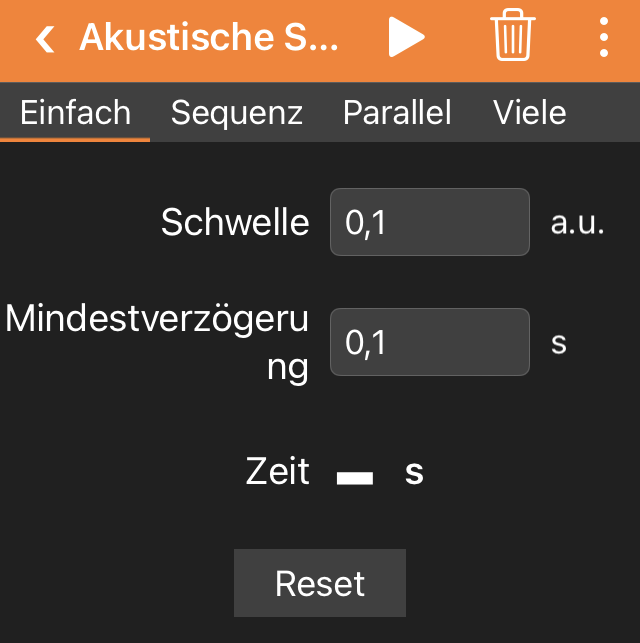
\includegraphics[width=\textwidth]{img/app}
    \end{minipage}

    \vspace{0.5cm}
    \textbf{Durchführung}: Zwei Personen stellen sich in einer Linie einen Schritt hinter die Handys und starten das Experiment. Beide Personen klatschen leicht zeitversetzt in die Hand. Person $A$ startet die Messung und Person $B$ stoppt die Messung an beiden Handys. Die gemessene Zeiten $t_A$ und $t_B$ werden notiert.

    \vspace{0.5cm}
    \textbf{Ergebnis}: Für die Zeit $t_A$ gilt
    \begin{align*}
        t_A = \Delta t_{AB} + t_B + \Delta t_{AB}
    \end{align*}
    Damit folgt
    \begin{align*}
        \Delta t_{AB} = \left | \frac{t_A-t_B}{2} \right | 
    \end{align*}
    Für die Schallgeschwindigkeit erhält man dann
    \begin{align*}
        c = \frac{l}{\Delta t_{AB}}
    \end{align*}

    \vspace{0.5cm}
    \textbf{Bemerkung}: Um zuverlässige Ergebnisse zu erhalten, ist es entscheidend, dass Handys und Personen möglichst eine Linie bilden.
\end{tcolorbox}


\end{document}
